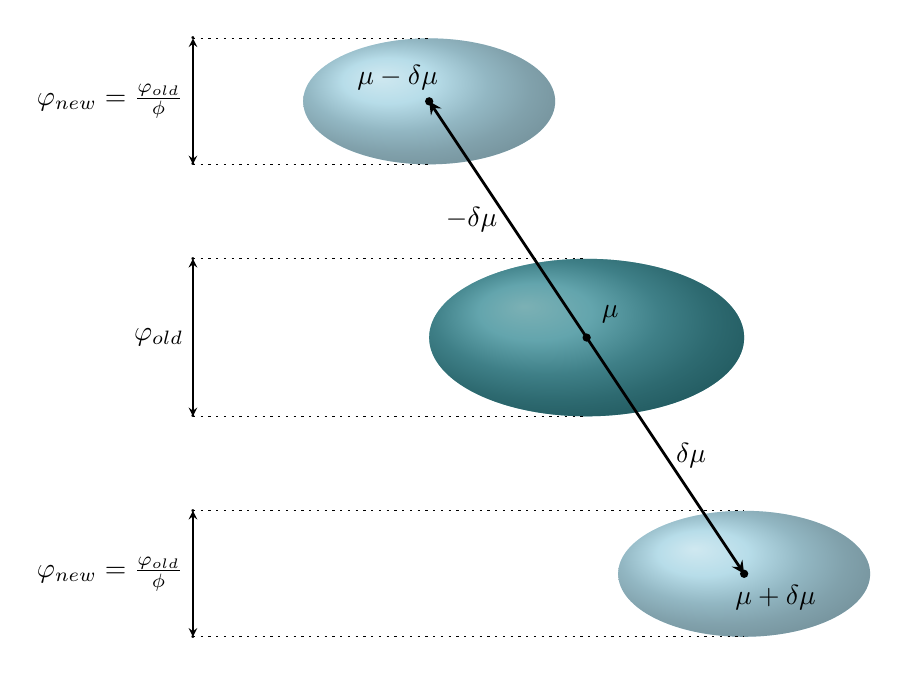
\begin{tikzpicture}
    \def\x{0}
    \def\y{2}
    \def\dx{2}
    \def\dy{-3}
    \def\s{1.25}
    \def\left{-5}
    \def\sx{2}
    \def\sy{1}
    \def\gop{0.5}
    \def\thickness{0.4}
    \definecolor{dark_cyan}{RGB}{5, 104, 110}
    \definecolor{light_cyan}{RGB}{173, 216, 230}
    % Draw the larger ellipse labeled X_μ
    \fill[dark_cyan] (\x, \y) ellipse ({\sx} and {\sy});
    \shade[ball color=light_cyan, opacity=\gop] (\x, \y) ellipse ({\sx} and {\sy});
    \fill (\x, \y) circle (1.5pt); % Point at the center of X_μ
    \node at (\x + 0.3, \y + 0.3) {\textbf{$\mu$}};

    % Draw the smaller dashed ellipse labeled "interior"
    \fill[light_cyan] (\x + \dx, \y + \dy) ellipse ({\sx / \s} and \sy / \s);
    \shade[ball color=light_cyan, opacity=\gop] (\x + \dx, \y + \dy) ellipse ({\sx / \s} and \sy / \s);
    \fill (\x + \dx, \y + \dy) circle (1.5pt); % Point at the center of X_μ

    \fill[light_cyan] (\x - \dx, \y - \dy) ellipse ({\sx / \s} and \sy / \s);
    \shade[ball color=light_cyan, opacity=\gop] (\x - \dx, \y - \dy) ellipse ({\sx / \s} and \sy / \s);
    \fill (\x - \dx, \y - \dy) circle (1.5pt); % Point at the center of X_μ
    % \node[below] at (0, -2.5) {\textit{interior}};

    % Draw points and arrow
    \draw[thick, ->, >=stealth, line width=1pt] (\x, \y) -- (\x + \dx, \y + \dy) node[midway, right] {$\delta \mu$};
    \draw[thick, ->, >=stealth, line width=1pt] (\x, \y) -- (\x - \dx, \y - \dy) node[midway, left] {$-\delta \mu$};
    \node at (\x + \dx + 0.4, \y + \dy - 0.3) {\textbf{$\mu + \delta \mu$}};
    \node at (\x - \dx - 0.4, \y - \dy + 0.3) {\textbf{$\mu - \delta \mu$}};
    
    % Annotate components of the formula
    \node at (\left, \y - \dy + \sy / \s) {.};
    \node at (\left, \y - \dy - \sy / \s) {.};
    \draw[thick, <->, >=stealth, line width=\thickness pt] (\left, \y - \dy + \sy / \s) -- (\left, \y - \dy - \sy / \s) node[midway, left] {$\varphi_{\text{new}} = \frac{\varphi_{\text{old}}}{\phi}$};
    \draw[thick, dotted, line width=\thickness pt] (\left, \y - \dy + \sy / \s) -- (\x - \dx, \y - \dy + \sy / \s);
    \draw[thick, dotted, line width=\thickness pt] (\left, \y - \dy - \sy / \s) -- (\x - \dx, \y - \dy - \sy / \s);

    \node at (\left, \y + \sy) {.};
    \node at (\left, \y - \sy) {.};
    \draw[thick, <->, >=stealth, line width=\thickness pt] (\left, \y + \sy) -- (\left, \y - \sy) node[midway, left] {$\varphi_{\text{old}}$};
    \draw[thick, dotted, line width=\thickness pt] (\left, \y + \sy) -- (\x, \y + \sy);
    \draw[thick, dotted, line width=\thickness pt] (\left, \y - \sy) -- (\x, \y - \sy);
    
    \node at (\left, \y + \dy + \sy / \s) {.};
    \node at (\left, \y + \dy - \sy / \s) {.};
    \draw[thick, <->, >=stealth, line width=\thickness pt] (\left, \y + \dy + \sy / \s) -- (\left, \y + \dy - \sy / \s) node[midway, left] {$\varphi_{\text{new}} = \frac{\varphi_{\text{old}}}{\phi}$};
    \draw[thick, dotted, line width=\thickness pt] (\left, \y + \dy + \sy / \s) -- (\x + \dx, \y + \dy + \sy / \s);
    \draw[thick, dotted, line width=\thickness pt] (\left, \y + \dy - \sy / \s) -- (\x + \dx, \y + \dy - \sy / \s);


\end{tikzpicture}